\chapter{Theoretical Framework}
\label{chap1}
\section{Introduction}
\label{chap1:intro}
How the world around was made? How does it work? These are fundamental questions asked a long-time ago to understand the Universe. The first efforts to elucidate those questions referred to ancient Greek philosophers. They gave much to physics by developing the fundamental basis of modern principles as the conservation of matter and the atomic theory. Democrats model introduced the notion of Atom as small indivisible building blocks (particles) of matter. At that moment, atoms described a variety of phenomena. \\
Rutherford came in 1909 with his experience demonstrating that atoms consist of mostly space with electrons surrounding a dense central nucleus (made up of protons and neutrons). At that time, Newtonian laws of motion and atoms provided a solid framework. A continuing collaboration between theorists and experimentalists brought us to a simple theory upon which all modern physic is based, the Standard Model (SM) of particle physics. Currently, SM is the most accurate model describing the universe composition. There are two types of elementary particles: the fundamental constituents of matter called "Fermions", and the quanta of fields called "Bosons" exchanged when an interaction occurs between fermions and bosons. The SM has successfully predicted the results from the measurements performed in the past 50 years. The following sections provide more details about the Standard Model and its particles.

\section{The Standard Model (SM) of particle physics}
\label{chap1:SM}
One of the physicist goals is to describe all natural phenomena with a minimal set of fundamental laws and theories which, at least in principle, quantitatively explain and predict experimental results. At the microscopic scale, all matter behaviour and phenomenology, including molecular, atomic, nuclear, and subnuclear physics, are explained under three fundamental interactions: electromagnetic, weak and strong forces. At the macroscopic scale, the fourth force, the gravitational interaction, has an essential role but is negligible at the microscopic scale. All the three interactions are described within a local relativistic Quantum Field Theory (QFT) based on the principal gauge invariance of SU(3)$\times$SU(2)$\times$U(1). This is "The Standard Model" of particle physics. Within the SM, matter consists of fermions and interactions are mediated by bosons. 

\subsection{Elementary Particles}
\label{chap1:SM:EP}
In the SM, particles are classified either as fermions or bosons depending on the associated statistics. Fermions obey to Fermi-Dirac statistics and respect the Pauli exclusion principle, i.e., two fermions in the same quantum state can not exist in the same place and time. Such particles have an intrinsic angular momentum, called spin J, equal to a half-integer. Bosons obey to Bose-Einstein statistics, due to the spin-statistics theorem, corresponding to integer spin value. Through an interaction, a boson emitted by a matter particle and then absorbed by another particle. Fermions are divided into two categories: Leptons and Quarks.

\subsubsection{Leptons}
Leptons whose name comes from the Greek word meaning "light", are grouped into three families or generations formed by three charged leptons: electron e, muon $\mu$ and tau $\tau$ with an electric charge -e, where e is equal to the elementary electric charge of $\sim 1.6 \ 10^{-19} $ C \cite{PDG}, and their neutral complemented partners neutrinos : $\nu_{e}, \nu_{\mu}$ and $\nu_{\tau}$. Only the electron and neutrinos are stable. A quantum number called Leptonic number (L) is associated with each lepton. Electron, muon, and tau have identical properties (e.g., charge, spin), however tau is 3477 times heavier than the electron while the muon is 17 times the mass of an electron. The rest mass of an electron is $9.10938356 \ 10^{-31} $ kg with a relative uncertainty of $3 \ 10^{-10}$. In high-energy physics, the particle mass is expressed in terms of its energy with the equivalence $E=mc^2$, where c is the light velocity in the vacuum, thus the electron mass is 511 keV.

\subsubsection{Quarks}
Quarks are electrically charged particles, with a charge of $+\frac{2}{3}e$ for the so-called up-type quarks and $-\frac{1}{3}e$ for the down-type quarks. There are six known quark flavours, similarly to leptons, quarks are paired into three generations. The first generation consists of up (u) and down (d) quarks, the second has the charm (c) and strange (s) quarks, and top (t) and bottom (b) quarks for the third generation. Quarks do not exist in a free state due to the QCD colour confinement.

Table \ref{tab:fermions} summarizes leptons and quarks. Each of the higher generations has particles with higher mass and tends to decay to the lower one, which explains why the ordinary matter made off the first-generation particles. Each fermion is associated with a corresponding anti-particle.
\begin{table}[htbp]
\centering
\begin{tabular}{lccc}
\hline\hline
 &
  1$^{st}$ Generation &
  2$^{nd}$ Generation &
  3$^{rd}$ Generation \\ \hline
\multicolumn{1}{c}{Quarks} &
  \begin{tabular}[c]{@{}c@{}}$u$\\ 2.16 MeV\\ $+\frac{2}{3}$\end{tabular} &
  \begin{tabular}[c]{@{}c@{}}$c$\\ 1.27 GeV\\ $+\frac{2}{3}$\end{tabular} &
  \begin{tabular}[c]{@{}c@{}}$t$\\ 172.4 GeV\\ $+\frac{2}{3}$\end{tabular} \\ \\ %\cline{2-4} 
\multicolumn{1}{c}{} &
  \begin{tabular}[c]{@{}c@{}}$d$\\ 4.67 MeV\\ $-\frac{1}{3}$\end{tabular} &
  \begin{tabular}[c]{@{}c@{}}$s$\\ 93 MeV\\ $-\frac{1}{3}$\end{tabular} &
  \begin{tabular}[c]{@{}c@{}}$b$\\ 4.18 GeV\\ $-\frac{1}{3}$\end{tabular} \\ \hline
\multicolumn{1}{c}{Leptons} &
  \begin{tabular}[c]{@{}c@{}}$e$\\ 0.511 MeV\\ -1\end{tabular} &
  \begin{tabular}[c]{@{}c@{}}$\mu$\\ 105.7 MeV\\ -1\end{tabular} &
  \begin{tabular}[c]{@{}c@{}}$\tau$\\ 1.8 GeV\\ -1\end{tabular} \\ \\ %\cline{2-4} 
\multicolumn{1}{c}{} &
  \begin{tabular}[c]{@{}c@{}}$\nu_{e}$\\ 0\\ 0\end{tabular} &
  \begin{tabular}[c]{@{}c@{}}$\nu_{\mu}$\\ 0\\ 0\end{tabular} &
  \begin{tabular}[c]{@{}c@{}}$\nu_{\tau}$\\ 0\\ 0\end{tabular} \\ \hline \hline
\end{tabular}
\caption{Generations of quarks and leptons with their masses and electrical charges}\label{tab:fermions}
\end{table}
The Standard Model of elementary particles assumes neutrinos to be mass-less, while some experiments demonstrate that neutrinos are changing flavours which can be explained by having a non-zero mass, which makes the SM an incomplete theory.

\subsubsection{Bosons}
As mentioned before, bosons are particles of integer angular momentum and obeying the Bose-Einstein statistics. They are the carriers of the gauge interactions between fermions. The photon ($\gamma$) is a boson known as a quantum of the electromagnetic field including electromagnetic radiation such as light. Photons are electrically neutral and mass-less particles. $W^{\pm}, Z^{0}$ are bosonic particles that carries the weak interaction. $Z^{0}$ boson is neutral while $W^{\pm}$ have a charge of $\pm$e. Contrary to photons, weak bosons are massive. $W^{\pm}$ and $Z^{0}$ have been predicted at the end of 1972 as the charged (CC) and neutral currents (CN) of the weak interaction. Their masses are predicted to be so large that it took many years to build powerful accelerators to produce them. They are directly observed at CERN in 1983 by the UA1 and UA2 collaborations \cite{UA1, UA2} and their masses were measured to be about 80 GeV and 91 GeV respectively. Gluons are the neutral quantum of the strong force known as the "glue" that links quarks to form hadrons. The mass of the gluons is known to be strictly zero.

\subsection{Elementary Interactions}
\label{chap1:SM:EI}
At the microscopic level, there are three fundamental forces: electromagnetic, weak and strong. The interactions with matter (fermions) is transmitted by boson. The SM content and interactions are expressed more formally through the concepts of symmetries and gauge invariance. Each interaction is described through a gauge group. The group generators correspond to the gauge bosons that are mediators of the fundamental force and responsible for the interactions. The electromagnetic interaction is mediated by photons, while the weak force have $W^{\pm}$ and $Z^{0}$ as mediators. The gluons are the mediators for the strong interaction.

\subsubsection{Electromagnetic interaction}
Quantum Electrodynamics (QED) describes the dynamics of electromagnetic interaction for electrically charged fermions and bosons. Each quantum field theory is represented by a Lagrangian density. The QED Lagrangian representing the behaviour of a freely propagating fermion field $\psi (x, t)$ is written as: 
\begin{equation}
    \mathcal{L} = \bar{\psi}i\gamma^\mu\partial_\mu\psi - m\psi\bar{\psi},
\end{equation}
where m is the particle mass. The Einstein convention is used here, with the indices $\mu= 0,1,2,3$ representing the space-time components x and the time t. \\ 
To be a valid gauge theory, the QED Lagrangian should be invariant under a U(1) (electromagnetic force group) local gauge transformation of the field: $\psi\rightarrow e^{i\alpha(x)}\psi$. This condition leads to additional terms to be added to the Lagrangian, a new gauge field $A_{\mu}$ that represents the photon:
\begin{equation}
    \mathcal{L}_{QED} = \bar{\psi}i\gamma^\mu\partial_\mu\psi - m\psi\bar{\psi} + q\psi\gamma^{\mu}\psi A_{\mu} - \frac{1}{4}F^{\mu\nu}F_{\mu\nu},
\end{equation}
where $F^{\mu\nu} = - F^{\mu\nu} = \partial^{\nu}A^{\mu} - \partial^{\mu}A^{\nu}$ is the field-strength tensor for the electromagnetic force which describes the kinetic propagation of the field. Note that U(1) is an Abelian group inducing that photons can not self-interact and the EM tensor does not have the photon self-interaction term included. The term $q\psi\gamma^{\mu}\psi A_{\mu}$ reflects the interaction between a fermion and the electromagnetic force (photon). The strength q (q=-e) is the electromagnetic interaction charge (electric charge). The mass term of the photon is not added to the Lagrangian since it spoils the gauge invariance. This is in agreement with the observation that the photon is mass-less. U(1) has one generator which corresponds to the photon mediator.

\subsubsection{Electro-Weak interaction}
The electroweak interaction consists of a unification of the electromagnetic and weak interactions. It is described by the combined gauge symmetry $SU(2)_{T}\times U(1)_{Y}$, where the $U(1)_{Y}$ symmetry mimics the QED one with the weak hypercharge Y. The $SU(2)$ represents the weak interaction with its generator vector T called weak isospin. The Lagrangian of the theory can be written as: 
\begin{equation}
    \mathcal{L}_{EW} = \bar{\psi}i\gamma^\mu\partial_\mu\psi -eY\bar{\psi}\gamma^{\mu}B_{\mu}\psi-g_{W}\bar{\psi}\gamma^{\mu}\textbf{T.W$_\mu$}\psi
    -\frac{1}{4}F^{\mu\nu}F_{\mu\nu} - \frac{1}{4}W^{i\mu\nu}W^i_{\mu\nu},
\end{equation}
where $g_{W}$ is the weak coupling to fermionic fields. The first two terms are similar to $\mathcal{L}_{QED}$. However, the term representing the coupling of fermions to photons is replaced by more general terms: the $W_{\mu}$ field and the hyper-photon $B_{\mu}$ field. The two charged vector bosons $W^\pm$ appear as a linear combination of the $W_{\mu}$ field components, $W^{\pm}_{\mu} = \frac{1}{\sqrt{2}}(W^1_{\mu}\mp W^2_{\mu})$. The photon is now created through the mixing of the $W_{\mu}$ and $B_{\mu}$ fields, as:
\begin{equation}
    A_{\mu} = B_{\mu}cos\theta_{W} + W^3_{\mu}sin\theta_{W},
\end{equation}
where $\theta_{W}$ is the weak mixing angle, and the $Z_{\mu}$ field, corresponding to the Z boson, is generated similarly as: 
\begin{equation}
     Z_{\mu} = -B_{\mu}sin\theta_{W} + W^3_{\mu}cos\theta_{W}.
\end{equation}
The field strength tensor for the weak gauge fields $W^i$ is defined as:
\begin{equation}
    W^{i}_{\mu\nu} = \partial_{\mu}W^i_{\nu} - \partial_{\nu}W^i_{\mu} - g_{W}\epsilon_{ijk}W^i_{\mu}W^i_{\nu},
    \label{eq:W}
\end{equation}
The non-Abelian nature of SU(2) group generates the third term in Eq. \ref{eq:W}, which gives rise to the weak boson self-interactions. \\
The electric charge q is related to Y and T through the Gell-Mann-Nishijima relation \cite{Gell}:
\begin{equation}
    q = T_3 + \frac{Y}{2},
\end{equation}
where $T_3$ is the third component of the isospin $T$.
Fermions are decomposed into left-handed and right-handed chirality types. The chirality is defined for mass-less particles as the same as helicity and refers to the relation between the spin and the momentum direction. For massive particles, chirality is trickier to define. Note that the electroweak force interacts only with left-handed particles because interaction with right-handed particles would violate the parity. The chirality separates left-handed doublets and right-handed singlets:
\begin{equation}
    (\nu_i \ i)^T_L, i_R \ \text{with} \ i = e, \mu \ or \ \tau,
\end{equation}
and, 
\begin{equation}
    (u \ d)^T_L, \ (c \ s)^T_L, \ (t \ b)^T_L, \ u_R, \ d_R ... \ . 
\end{equation}

\subsubsection{Strong interaction}
Additionally to QED, the strong interaction is described by Quantum Chromodynamics (QCD), which is a local gauge symmetry under $SU(3)_C$. SU(3) has eight generators corresponding to the eight gluons mediators of the strong force. The expression for the locally gauge invariant Lagrangian of the QCD, which describes interactions of quarks of mass m and quark-field spinors $\psi$ via mass-less gluons is:
\begin{equation}
    \mathcal{L}_{QCD} = \sum_{flavours} \bar{\psi}_a(i\gamma^\mu\partial_\mu\delta_{ab}-g_{s}\gamma^\mu t^C_{ab}G^C_\mu - m\delta_{ab})\psi_b - \frac{1}{4}F^A_{\alpha\beta}F^{A\alpha\beta},
\end{equation}
where a = 1,2,3 is the colour index. The $G^{C}_\mu$ are the gluon fields with C= 1,2,...,8 referring to the eight gluons. The $t^C_{ab}$ are the generators of the SU(3) group. The quantity $g_{s}$ corresponds to the strong coupling constant that determines the strength of interactions between coloured particles (quarks and gluons). The strong field tensor is defined as:
\begin{equation}
    F^A_{\alpha\beta} = \partial_\mu G^A_\nu - \partial_\nu G^A_\mu - g_sf^{ABC}G^B_\mu G^C_\nu,
\end{equation}
where $f^{ABC}$ are the structure constants of the SU(3) group. In contrast to QED, the field tensor of the QCD includes the gluon triplet and quartic self-interaction. Only particles carrying colour charge (i.e. quarks) couple to these gluons. Colour charge is conserved in each interaction. Since the SU(3) group is non-Abelian, the gluons themselves must carry (anti-)colour charge and thus interact with each other. \\
Finally, the Standard Model Lagrangian density could be summarized as: 
\begin{equation}
    \mathcal{L}_{SM} \sim \mathcal{L}_{EW} + \mathcal{L}_{QCD}.
\end{equation}
Note that, in the $\mathcal{L}_{EW}$ no mass term is introduced for the two W/Z appearing bosons, while experimental observations indicate large masses for them. Additionally, the fermion mass term that appeared in $\mathcal{L}_{QED}$ is now absent in $\mathcal{L}_{EW}$, requiring the introduction of an additional mechanism to explain the origin of their mass. The introduction of terms related to mass is handled through the process of Electroweak Symmetry Breaking (EWSB), and the introduction of the Higgs boson mechanism.

\section{Electroweak Symmetry Breaking (EWSB)}
\label{chap1:EWSB}
The gauge bosons mass terms cannot be simply introduced as they would break gauge invariance. In 1964, the Brout-Englert-Higgs (BEH) mechanism introduced a spontaneous symmetry breaking ad-hoc in the SM to preserve the local gauge invariance \cite{Englert} called Electroweak Symmetry Breaking (EWSB). In this minimal model, the mass of the particle is generated by introducing the Higgs field represented by a weak isospin doublet of one charged and one neutral complex scalar (J=0) field:
\begin{equation}
    \phi(x)=\frac{1}{\sqrt{2}}\left(\begin{array}{c}
\phi_{+} \\
\phi_{0}
\end{array}\right).
\end{equation}
The Higgs Lagrangian is added to the SM Lagrangian as:
\begin{equation}
    \mathcal{L}_{\mathrm{Higgs}}=\left(D^{\mu} \phi\right)^{\dagger}\left(D_{\mu} \phi\right)-V(\phi),
\end{equation}
where $D^\mu$ is the covariant derivative $D^\mu =\left(\partial_{\mu}+i g T^{i} W_{\mu}^{i}+i \frac{1}{2} g^{\prime} B_{\mu}\right)$. The kinetic and the interaction of the Higgs field with weak gauge bosons is described by the term $D^\mu\phi$. $V(\phi)$ is the Higgs potential:
\begin{equation}
    V(\phi)=\mu^{2} \phi^{+} \phi+\lambda\left(\phi^{+} \phi\right)^{2},
\end{equation}
the first term is associated with the mass of the field and the second represents the quadratic self-interaction of the scalar field. The parameter $\lambda$ has to be positive to obtain a potential with finite minima, while $\mu$ can be chosen freely. For $\mu^{2} > 0$, the potential has a single ground state at zero with all fields being zero ($\phi_0 = 0$). Hence, the vacuum expectation value of the Higgs field would be zero and the symmetry is preserved. However, for $\mu^{2} < 0$ the potential has an infinite set of minima $v$ given by:
\begin{equation}
    \phi_{0}=<\phi^{+} \phi>=\frac{v^{2}}{2}=-\frac{\mu^{2}}{2 \lambda},
\end{equation}
$v\neq0$ being the vacuum expectation value (vev) which is illustrated in Figure \ref{fig:chap1:Higggs_potential}.
\begin{figure}[htbp]
    \centering
    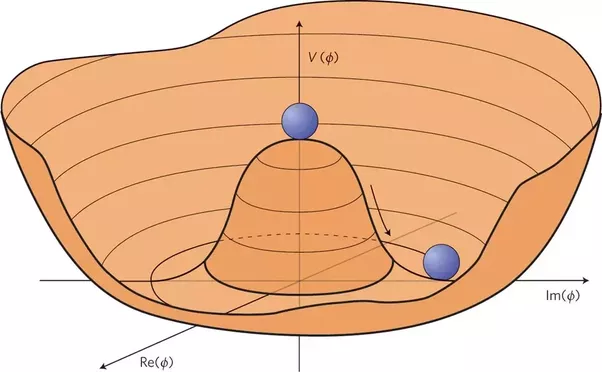
\includegraphics[width=0.5\textwidth]{Ch1/Img/Higgs_potential.png}
    \caption{Shape of the Higgs potential for $\mu^{2} < 0$. This potential has an infinite amount of minima. \cite{HiggsPotential}}
    \label{fig:chap1:Higggs_potential}
\end{figure}

The choice of the physical vacuum state spontaneously breaks the Lagrangian symmetry. An expansion of $\phi_0$ around its vacuum state $v$ introduces a massive scalar and three mass-less Goldstone bosons. However, the Goldstone bosons appear to be not physical and can be eliminated using the gauge Unitary, enforcing the Higgs doublet to be real:
\begin{equation}
    \phi(x)=\frac{1}{\sqrt{2}}\left(\begin{array}{c}
0 \\
v+h(x)
\end{array}\right),
\end{equation}
where $h(x)$ is the physical field linked to a new massive particle: the Higgs boson. \\
The form of Higgs potential becomes: 
\begin{equation}
    V(\phi)=-\frac{1}{2} m_{H}^{2} h^{2}(x)+\lambda_{H H H} h^{3}(x)+\lambda_{H H H H} h^{4}(x),
\end{equation}
where $m_{H}^{2}=2 \lambda^{2}=2 \lambda v^{2}$ is the square of Higgs boson mass, $\lambda_{HHH}$ is the coupling in a vertex with tree Higgs bosons (trilinear coupling) and $\lambda_{HHHH}$ for the case of four Higgs bosons.
Accordingly, the terms giving the mass to the gauge bosons can be identified:
\begin{equation}
m_{W} = \frac{1}{2}gv 
\end{equation}
\begin{equation}
m_{A} = 0    
\end{equation}
\begin{equation}
m_{Z} = \frac{m_{W}}{\cos\theta_{W}}.
\end{equation}
The Higgs mechanism associates the degrees of freedom of the hypothetical scalar (Goldstone) bosons with the longitudinal components of gauge bosons and consequently become massive. The coupling of the Higgs boson to the gauge bosons appears to be proportional to the gauge boson masses. The mass of the fermions cannot be explained in the same way as the fermions acquire masses through the corresponding Yukawa couplings. Weak bosons masses are predicted in the SM, while Higgs boson mass is unknown and can not be constrained from other SM measurement. The Higgs boson discovery is necessary to confirm the EWSB \cite{EWSB}, and the Higgs boson properties needs to be measured.

\section{Higgs boson : Production and observation}
\label{chap1:H2012}

\subsection{Previous searches for Higgs boson}

The Large Electron-Positron (LEP) collider, approved by the CERN Council in 1981 and commissioned eight years later, provided a detailed study of the electroweak interaction until 2000. It accelerated and collided electron and positron beams at a centre-of-mass energy $\sqrt{s}$ from 91 to 200 GeV. Its results have been used to perform stringent tests of the SM by comparing the precise measurements with theory predictions. This checked the correctness of the SM theory. Observing the Higgs boson was of particular interest because this fundamental ingredient of SM has not been observed and needed to complete the SM picture. \\
At the beginning of the LEP program, no solid prediction existed on the mass of the Higgs boson. Searches for the SM Higgs boson carried out by the four LEP experiments extended the sensitive range well beyond that anticipated. Similarly, the Tevatron experiments CDF and D0 have excluded a range of mass $162 < m_{H} < 166$ GeV. Tevatron was a proton-antiproton ($p\bar{p}$) collider at a centre-of-mass energy of 3 TeV. Figure \ref{fig:chap1:H2012:LEP} shows the LEP and Tevatron exclusion limits \cite{LEP, Tevatron, LEP_Tevatron}. Combination of LEP and Tevatron results yields to the best estimated Higgs boson mass at that time of $m_{H} = 116.4^{+15.6}_{-1.3}$ GeV. 
\begin{figure}[htbp]
    \centering
    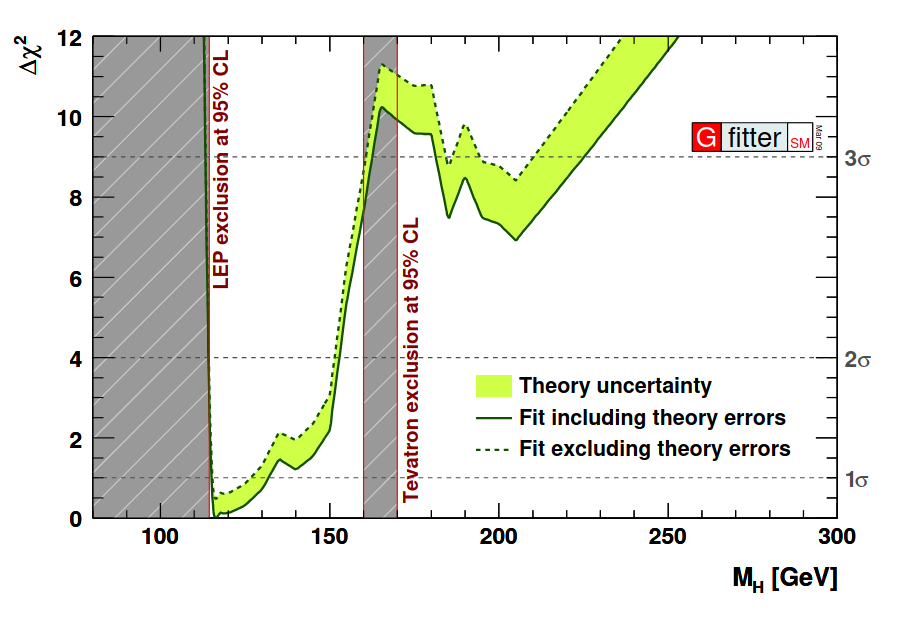
\includegraphics[width=0.5\textwidth]{Ch1/Img/LEP_Tevatron_limits.png}
    \caption{The $\chi^2$ function for the SM as a function of the Higgs boson mass, LEP and Tevatron exclusions limits are shown.}
    \label{fig:chap1:H2012:LEP}
\end{figure}
\\
This is due to the higher energy achieved and to more sophisticated detectors and analysis techniques. However, circular accelerators with electrons are limited by synchrotron radiation due to the small electron mass. Since muon acceleration is not technically possible at the current stage due to the short lifetime of the muon, proton collisions with accelerator technology represented a good way to achieve high-energy collisions needed for Higgs boson discovery. \\
LHC provides a nominal proton-proton collision at a centre-of-mass energy $\sqrt{s}$ up to 14 TeV. But at the beginning of LHC the energy was limited to 7-8 TeV for safety reason on the accelerator. During the last four years, the achieved energy is 13 TeV. LHC is detailed in the dedicated Chapter \ref{LHC&ATLAS}. 
\subsection{Proton-proton collisions}
\label{chap1:H2012:PP}
Protons are fermions made of two up and one down quarks ($uud$) called "valence" quarks. They interact with each other through the strong force via gluon exchange. Due to the nature of QCD (non-abelian), gluons can fluctuate into quark anti-quark pairs forming the so-called "sea" quarks. Effectively, a proton is therefore a bound state of quarks and gluons called partons each carries a fraction $x$ of the total proton momentum. At the LHC, process are produced by colliding mainly protons beams. The Higgs boson is produced in a proton-proton collision as:
\begin{equation}
    p_1 + p_2 \rightarrow H.
\end{equation}
The probability for a process to occur is expressed in terms of its cross-section, and the dynamic of its products is determined by the dynamics of partons involved in the collision. The hard scattering cross-section for such a process is given by:
\begin{equation}
    d \sigma^{p_{1} p_{2} \rightarrow H}=\int_{0}^{1} d x_{1} \int_{0}^{1} d x_{2} \sum_{a, b} f_{a / p_{1}}\left(x_{1}, \mu_{F}^{2}\right) f_{b / p_{2}}\left(x_{2}, \mu_{F}^{2}\right) d \hat{\sigma}^{a b \rightarrow H}\left(x_1, x_2, \mu_{F}^{2}\right), 
\end{equation}
where $a$, $b$ are the partons involved in the process and $f_{n/p_i}(x_i)$ is the parton distribution function (PDF), which is the probability to find a parton of type $n$ inside the proton $p_i$ with a longitudinal momentum fraction $x_i$ at the energy scale $Q$. $\sigma^{a b \rightarrow H}$ is the parton cross-section of the process. \\
In general, the x dependence at a given $Q^2$ cannot be calculated analytically but rather are extracted from global fits to data from many experiments. Different parton distribution function sets use different fitting methods and experimental data \cite{PDF}. Figure \ref{fig:chap1:H2012:PDF} shows two examples of CT14 parton distribution functions at different $Q^2$ computed using data from LHC experiments, and the new D\O \ charged lepton rapidity asymmetry data \cite{CT14}. 
\begin{figure}[htbp]
    \centering
    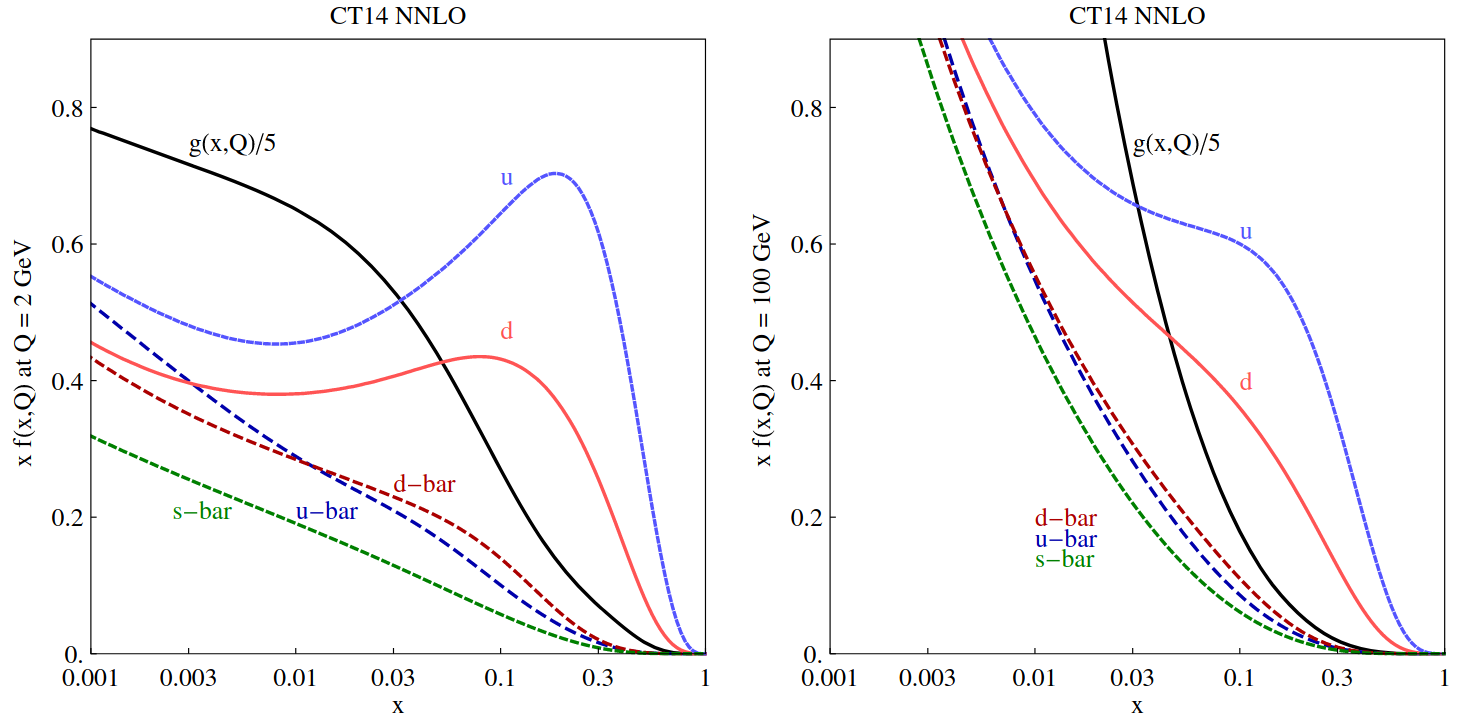
\includegraphics[width=0.7\textwidth]{Ch1/Img/pdf_CT14_NNLO.png}
    \caption{The CT14 PDFs at Q=2 GeV (left) and Q = 100 GeV (right) for different partons. These PDFs are computed at the next-to-next-to-leading order.}
    \label{fig:chap1:H2012:PDF}
\end{figure}
The production of the Higgs boson at the LHC occurs in different modes. Their cross-sections depend on the coupling of the Higgs boson to specific particles, but also essentially on the PDFs described above.

\subsection{Higgs boson production}
\label{chap1:EWSB:HP}
The main processes contributing to the Higgs boson production at LHC are represented by their leading Feynman diagrams displayed in Figure \ref{fig:chap1:EWSB:HP}. 
\begin{figure}[htbp]
    \centering
    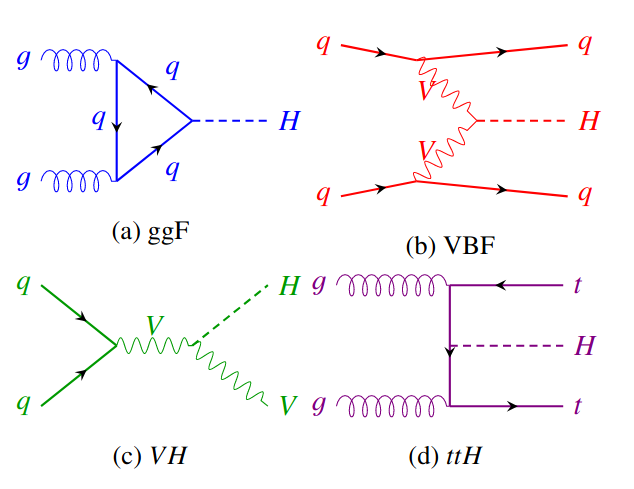
\includegraphics[width=0.5\textwidth]{Ch1/Img/Higgs_prod_modes.png}
    \caption{Feynman diagrams for the main production modes of Higgs boson.}
    \label{fig:chap1:EWSB:HP}
\end{figure}
In the 7-13 TeV centre-of-mass energy range, the most important Higgs boson production is the fusion of gluons (ggF).\\
In order of decreasing cross-section as shown in Figure \ref{fig:chap1:EWSB:HXSEC} (a), the Higgs boson production modes are:
\begin{itemize}
	\item Gluon-gluon fusion (ggF): the main Higgs boson production at LHC. The process involves the fusion of two incoming gluons that produce the Higgs boson through a heavy quark loop, whose main contribution comes from the top quark. The corresponding Feynman diagram is shown in Figure \ref{fig:chap1:EWSB:HP} (a).  
	\item Vector Boson Fusion (VBF): each of the two interacting quarks emit a $W^{\pm}$ or $Z^0$ boson which, in turn, interact to produce the Higgs boson, as shown in figure \ref{fig:chap1:EWSB:HP} (b). Quarks deriving from the incoming partons after the emission of vector bosons proceed in the forward direction and represent the peculiar signature of this production mode, two high-energy forward jets separated by a large pseudo-rapidity gap, a $\Delta\eta$ region with reduced particle density. This process has a cross-section which is one order of magnitude lower than ggF, and it would have become comparable to ggF for Higgs boson mass of the order of 1 TeV as shown in Figure \ref{fig:chap1:EWSB:HXSEC} (b).
	\item Vector boson associated production (VH): also known as Higgs-strahlung, this process is characterized by the emission of a Higgs boson from a $W^{\pm}$ or $Z^0$ boson produced by two incoming quarks, as shown in figure \ref{fig:chap1:EWSB:HP} (c). The VH cross-section is several orders of magnitude lower than the ggF and VBF cross-sections for $m_H$ larger than about 300 GeV, while the VH and VBF cross-sections are comparable around $m_H = 125$ GeV as shown in Figure \ref{fig:chap1:EWSB:HXSEC} (b).
	\item Top quark associated production ($t\bar{t}H$): a pair of top quarks, originated from the splitting of two incoming gluons, interacts to give rise to a Higgs boson, as shown in figure \ref{fig:chap1:EWSB:HP} (d). The production in association with a pair of top quarks allows a direct measurement of the Higgs boson coupling to the top quark. Another production mechanism analogous to the $t\bar{t}H$ process and with a similar cross-section is the b-quark associated production.
\end{itemize}
The SM Higgs boson production cross-section for the various production modes depends on the Higgs boson mass and the centre-of-mass energy, as shown in Figure \ref{fig:chap1:EWSB:HXSEC}. 
\begin{figure}[htbp]
    \centering
    \subfloat[][]{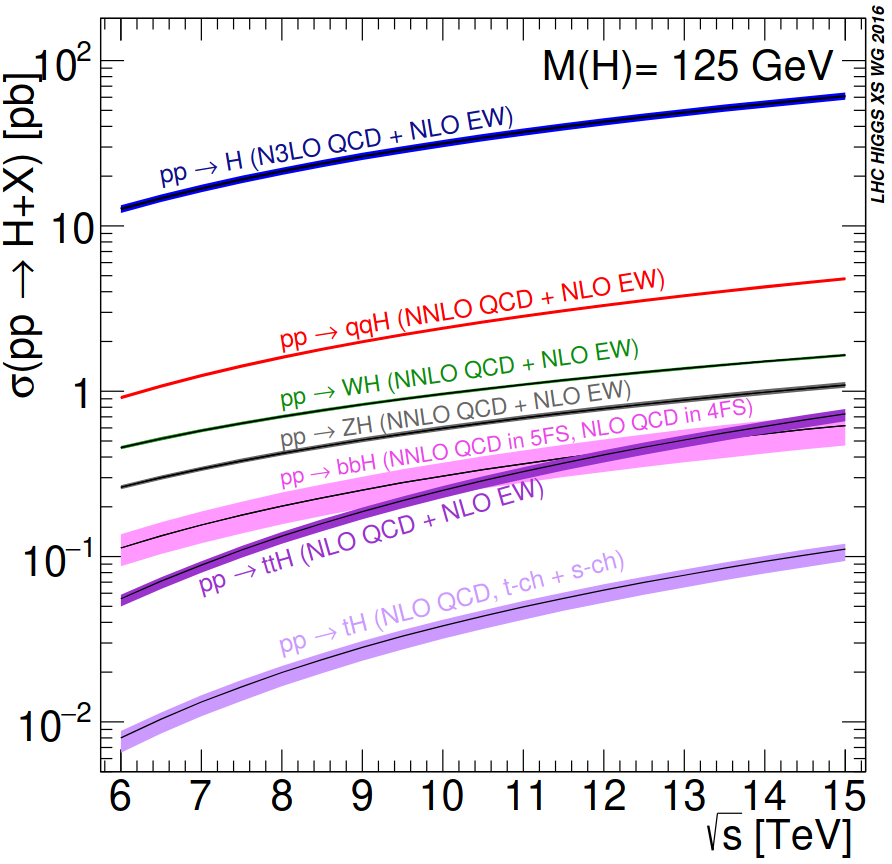
\includegraphics[width=.45\textwidth]{Ch1/Img/Higgs_Xsec_s.png}}
    \subfloat[][]{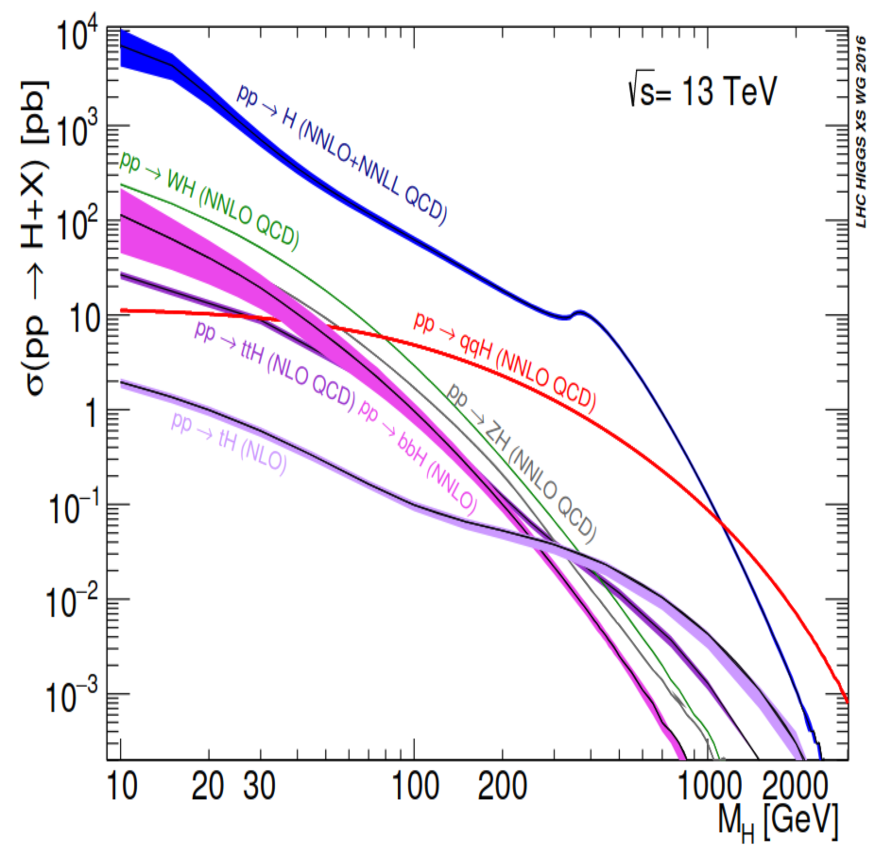
\includegraphics[width=.46\textwidth]{Ch1/Img/Higgs_Xsec_mass.png}}
    \caption{Cross-sections for different Higgs boson production modes at a proton-proton collider with a centre-of-mass energy of 6-15 TeV (a). A Higgs boson mass of 125 GeV is assumed in this plot. Additionally, cross-sections as a function of Higgs boson mass are shown (b) \cite{LHCHXSWG_Twiki}.}
    \label{fig:chap1:EWSB:HXSEC}
\end{figure}
The Higgs boson is an unstable particle as shown in Figure \ref{fig:chap1:EWSB:D}. Note that the probability to decay within a given time "decay width" $\Gamma$ is linked to the lifetime $\tau$ by $ \Gamma\tau = \hbar$ where $\hbar$ is the reduced Planck constant. The Higgs boson decay width for a Higgs boson mass $m_{H} = $ 125 GeV is around 4 MeV \cite{CMS_HiggsWidth}.
\begin{figure}[htbp]
    \centering
    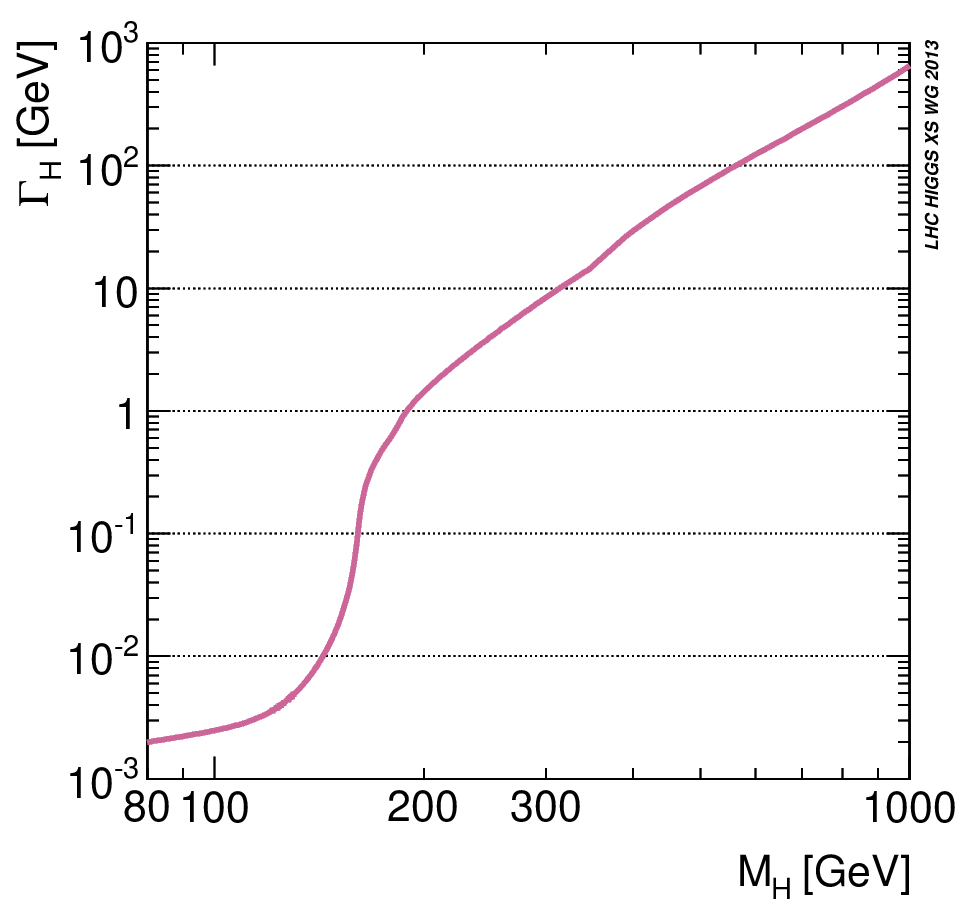
\includegraphics[width=0.45\textwidth]{Ch1/Img/Higgs_decay.png}
    \caption{Higgs boson total decay width as a function of Higgs boson mass \cite{HiggsWidth}.}
    \label{fig:chap1:EWSB:D}
\end{figure}
\\
In order to identify the Higgs boson and its production modes, it is reconstructed from its products for a chosen decay channel. 


\subsection{Higgs boson decay channels}
\label{chap1:EWSB:HD}
The possible SM Higgs boson decay modes are very dependent on the Higgs boson mass as shown in Figure \ref{fig:chap1:EWSB:BR}. If the Higgs boson was heavy enough to decay into two real vector bosons, the modes $H\rightarrow WW^*$ and $ H\rightarrow ZZ^*$ would have dominated the decay with small contribution from Higgs boson to di-top quarks. At very low masses of the Higgs boson, decays into the vector boson or $t\bar{t}$ would have played almost no role and the dominant decay mode would have been the experimentally challenging decay mode $H\rightarrow b\bar{b}$.
\begin{figure}[htbp]
    \centering
    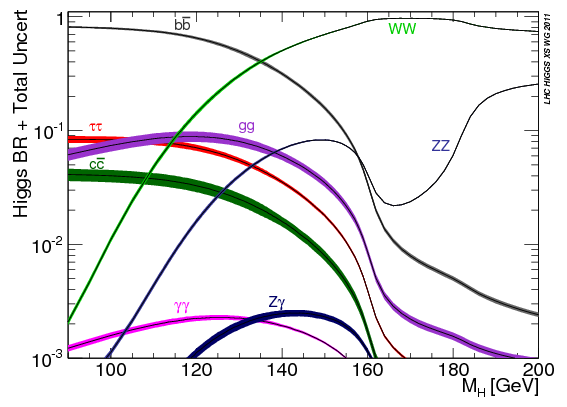
\includegraphics[width=0.5\textwidth]{Ch1/Img/Higgs_Br.png}
    \caption{Higgs boson branching ratio of the possible Higgs boson decay channels as a function of the Higgs boson mass \cite{HiggsBR}}
    \label{fig:chap1:EWSB:BR}
\end{figure}
Since photons are mass-less particles, the direct coupling of the Higgs boson to photons is zero in the SM. However, the Higgs boson can decay into a pair of photons via loop processes. The main Feynman diagrams of this decay are shown in Figure \ref{fig:chap1:EWSB:Hgg}. 
At a Higgs boson mass of 125 GeV, the dominant decay of the Higgs boson is $H \rightarrow b\bar{b}$ with a branching ratio of roughly 58\%. At the same mass $H\rightarrow\gamma\gamma$ branching ratio is around 0.23\% \cite{HXSWG}.
\begin{figure}[htbp]
    \centering
    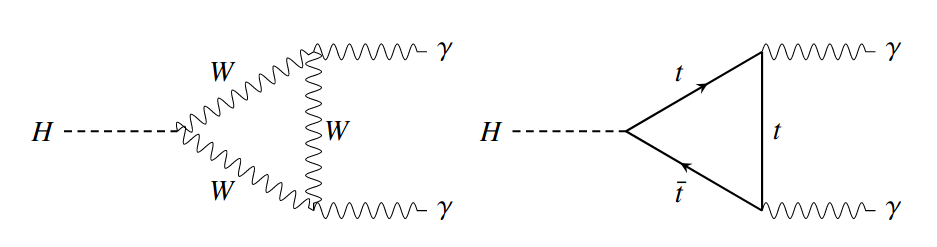
\includegraphics[width=0.5\textwidth]{Ch1/Img/H_to_gammagamma.png}
    \caption{Feynman diagrams of the $H\rightarrow\gamma\gamma$ decay. Other particles can also contribute to the loop.}
    \label{fig:chap1:EWSB:Hgg}
\end{figure}

\subsection{Higgs boson discovery}
\label{chap1:H2012:HM}
The ATLAS and CMS collaborations, located at the LHC collider, announced on 4 July 2012 the identification with a confidence of $5\sigma$ of a new boson within a mass range of 125-127 GeV \cite{ATLAS_2012, CMS_2012}. The new boson was consistent with the Standard Model Higgs boson decay modes and signal rate. Later, it was confirmed that the new particle corresponds to the Higgs boson. The Higgs boson was predicted in 1964, but the world had to wait until 2012 for its discovery. The evidence of the new boson was performed in the three bosonic decay channels $H\rightarrow ZZ^* \rightarrow 4l, H\rightarrow\gamma\gamma$ and $H\rightarrow WW^*\rightarrow l\nu l\nu$. The $H\rightarrow\gamma\gamma$ has a small branching ratio, while the reconstruction of the two photons has a clean signature in the detector which allows for a good photon energy resolution. This signal is therefore well separated from the dominating continuum background from the QCD $\gamma\gamma$+jets, which has a smooth and well parametrisable shape. This makes the $H\rightarrow\gamma\gamma$ decay mode one of the most sensitive channel.

Events collected in 2010 and 2011 with centre-of-mass energy $\sqrt{s}=$ 7 TeV and 8 TeV respectively, containing two photons were combined. Figure \ref{fig:chap1:H2012:Hyy} shows the distribution of the invariant mass of photon pairs measured by ATLAS experiments, and demonstrates a statistically significant excess of events near 125 GeV. 
\begin{figure}[htbp]
    \centering
    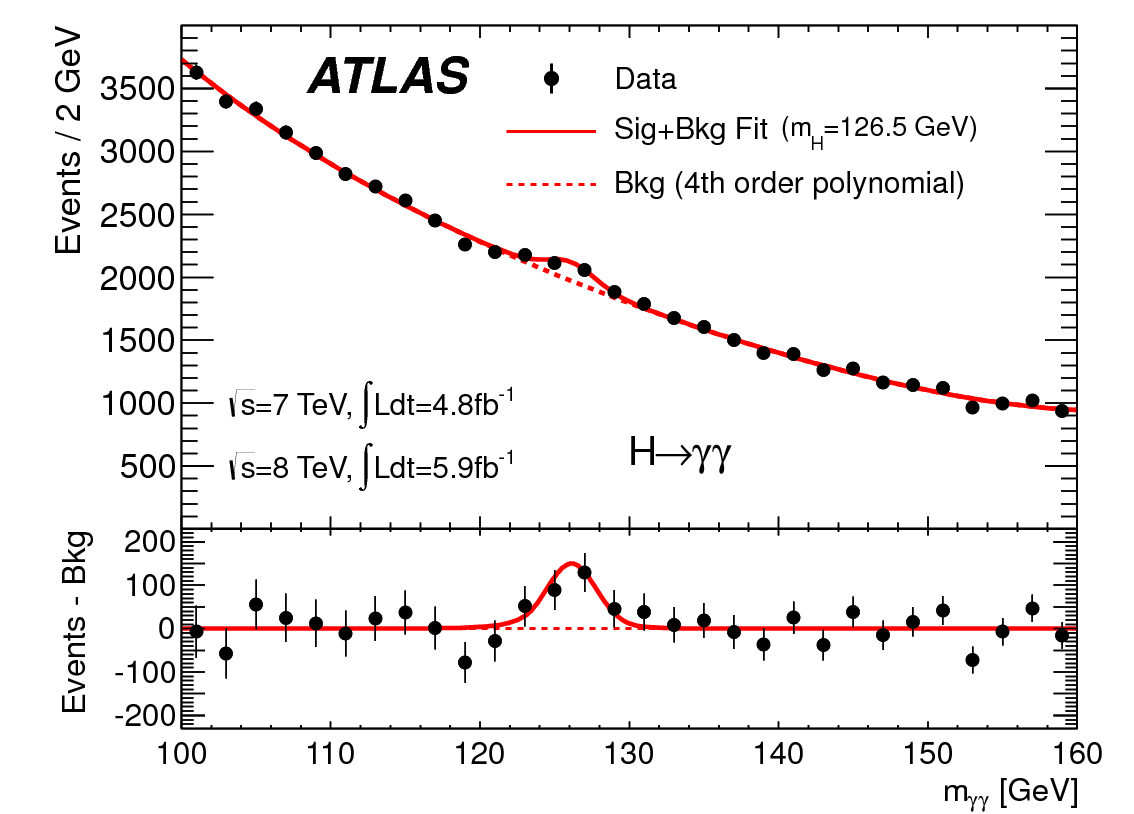
\includegraphics[width=0.5\textwidth]{Ch1/Img/Hmyy.png}
    \caption{Distributions of the invariant mass of di-photon system \cite{ATLAS_2012}.}
    \label{fig:chap1:H2012:Hyy}
\end{figure}
\\
Measurements of the three bosonic channels were combined to confirm the observation of the new particle \cite{ATLAS_2012}. The observed local significance reaches $6\sigma$ (the observed signal is $\sim10^{-9}$ to be a background fluctuation) around 125 GeV making the first observation of the Higgs boson, as shown in Figure \ref{fig:chap1:H2012:P0}.
\begin{figure}[htbp]
    \centering
    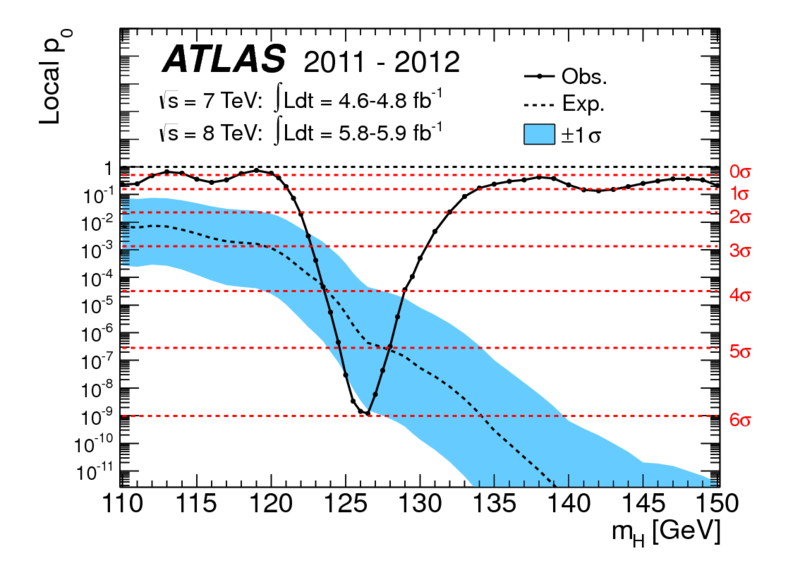
\includegraphics[width=0.5\textwidth]{Ch1/Img/Hp0.png}
    \caption{The observed local p-value as a function of $m_H$ (solid line) and the expectation with its $\pm1\sigma$ band assuming the presence of a Standard Model Higgs boson at that mass (dashed line) from the combination of the $ZZ^*$ and  $\gamma\gamma$ channels by the ATLAS experiment. The horizontal dashed lines indicate the p-values corresponding to significance of 1 to 6$\sigma$ \cite{ATLAS_2012}.}
    \label{fig:chap1:H2012:P0}
\end{figure}
\\
The latest measurement of the Higgs boson using the data collected during 2015-2018 corresponding to 139 \ifb yields to a mass of $m_{H}=125.09 \ \pm \ 0.24 $ GeV \cite{Mass}. Figure \ref{fig:chap1:H2012:MyyRun2} shows the diphoton invariant mass distribution of event collected during 2015-2018. Figure \ref{fig:chap1:H2012:HXsecRun2} shows the best-fit values of the production cross-sections times branching fraction in the different channel to their SM values.
\begin{figure}[htbp]
    \centering
    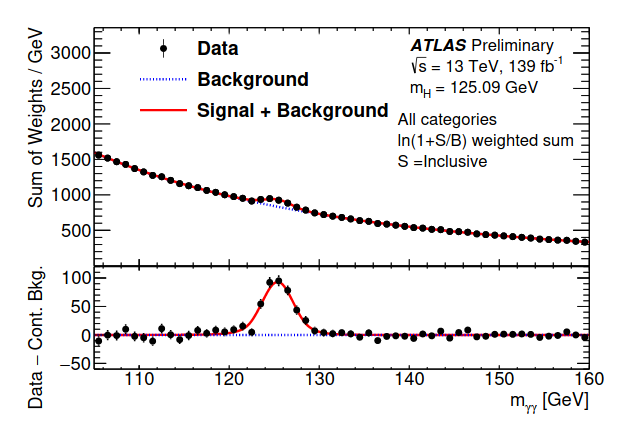
\includegraphics[width=0.5\textwidth]{Ch1/Img/myy_run2.png}
    \caption{The inclusive diphoton invariant mass distribution \cite{ATLAS_2020}.}
    \label{fig:chap1:H2012:MyyRun2}
\end{figure}
\begin{figure}[htbp]
    \centering
    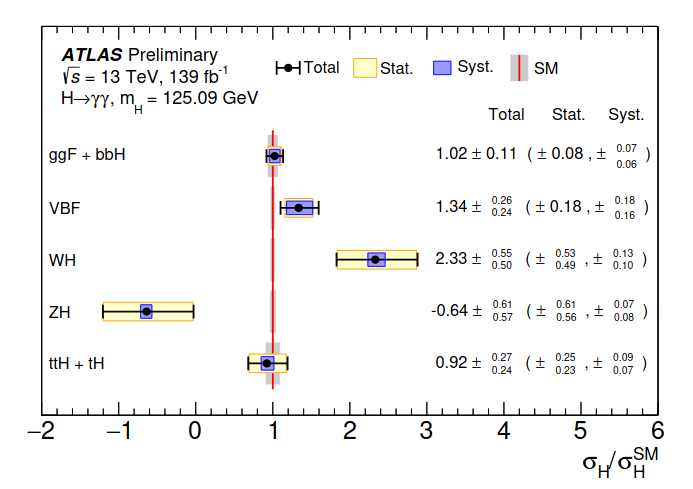
\includegraphics[width=0.5\textwidth]{Ch1/Img/HXsecRun2.png}
    \caption{Cross-section times branching fraction for $ggF+b\bar{b}H , \ VBF, \ VH$ and $t\bar{t}H + tH$ production, normalized to their SM predictions \cite{ATLAS_2020}.}
    \label{fig:chap1:H2012:HXsecRun2}
\end{figure}
\\

Finally, by the observation of the Higgs boson, the last piece of the standard model of elementary particles was found. SM particles are summarized in Figure \ref{fig:chap1:H2012:SM}. 
\begin{figure}[htbp]
    \centering
    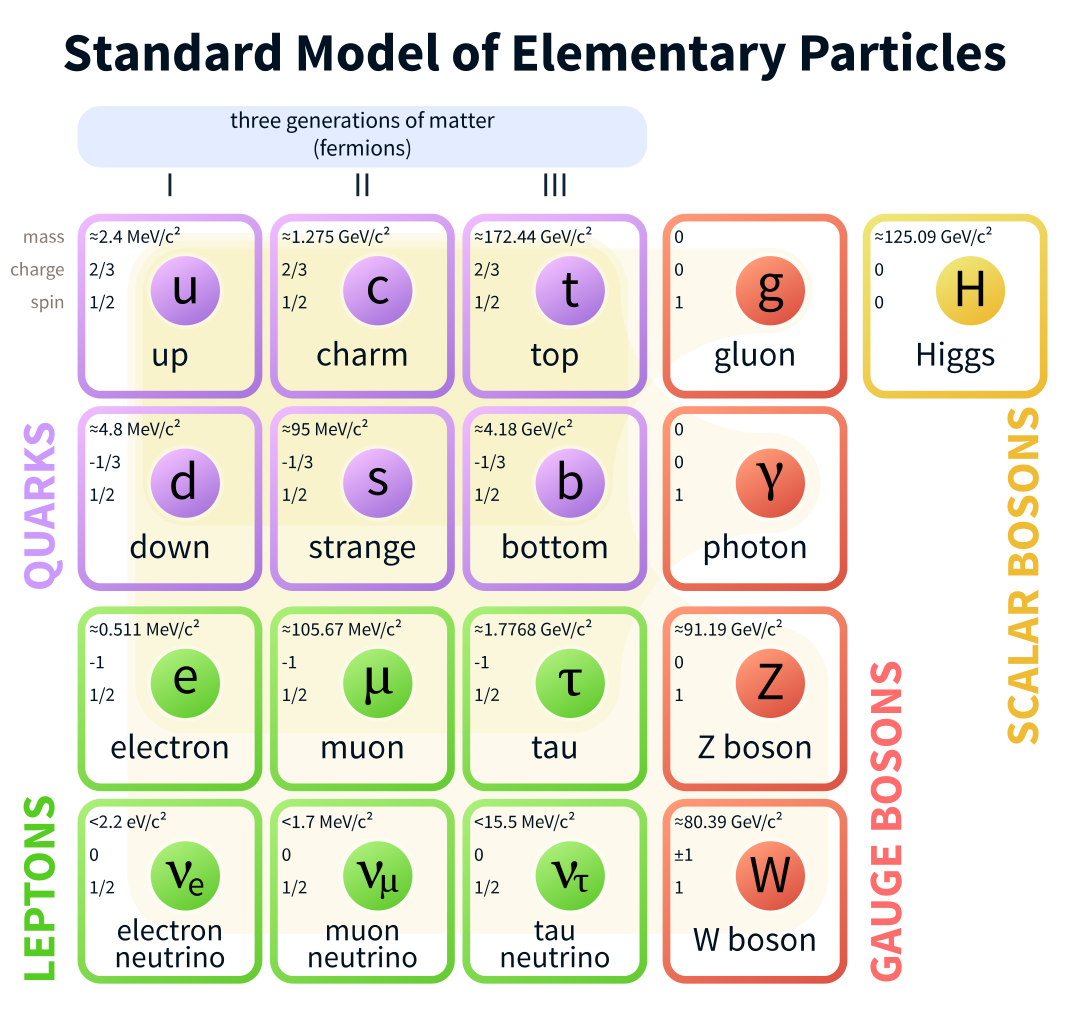
\includegraphics[width=0.5\textwidth]{Ch1/Img/SM_particles.png}
    \caption{The particle content of the standard model of particle physics.}
    \label{fig:chap1:H2012:SM}
\end{figure}
\\
Measuring the properties and couplings of the last piece of SM is a priority for both ATLAS and CMS. Higgs boson self-couplings $\lambda_{HHH}$ is vital, providing a direct probe on the EWSB and is a precision test of the electroweak theory. A direct probe of the trilinear coupling is possible through studying Higgs boson pair production where two Higgs bosons are produced in the same event, making di-Higgs boson analyses particularly interesting and the main subject of this thesis.
\clearpage
\section{Looking for di-Higgs boson events}
\label{chap1:HH}
Double Higgs boson production (HH) presents the only direct probe of the Higgs boson self-coupling. Confirming the existence and amplitude of the Higgs boson self-coupling is one of the main key prediction of the SM not observed yet. In particular, the measurement of the Higgs boson self-coupling $\lambda$ (also referred to as the Higgs boson trilinear coupling $\lambda_{HHH}$) is of great importance to yield a deeper understanding of particle physics and cosmology. This measurement makes it possible to experimentally reconstruct the Higgs potential and check whether the Higgs boson discovered in 2012 at CERN is the one predicted by the Brout-Englert-Higgs mechanism. The di-Higgs boson production rate gives a handle to measure more accurately the Higgs potential. The main goal of this thesis is the search of Higgs boson pair production.
\subsection{Di-Higgs boson production and decays} 
\label{chap1:HH:HPD}
As the SM provides the trilinear coupling of the Higgs boson, all SM Higgs boson production modes are known for di-Higgs boson production. Similarly to the single Higgs boson, HH production is dominated by gluon-gluon fusion (ggF) through the destructive interference of two LO Feynman diagrams, shown in Figure \ref{fig:chap1:HH:HPD:FY}, involving top-quark loops and the triple Higgs boson self-coupling. In the box diagram, the top-quark Yukawa coupling \textcolor{blue}{$\lambda_t$} is present in two vertices so the contribution of this diagram to the amplitude is proportional to $\lambda_t^2$. In the triangle diagram, there is $\lambda_t$ in one vertex and the triple Higgs boson self-coupling \textcolor{red}{$\lambda_{HHH}$} in the other vertex, thus the contribution of this diagram is proportional to $\lambda_t\cdot\lambda_{HHH}$. The amplitude of the process can be written as:
\begin{equation}
    A(\lambda_t, \lambda_{HHH}) \equiv \lambda_t^2\cdot\square + \lambda_t\cdot\lambda_{HHH}\bigtriangleup,
\end{equation}
where $\square$ represents the contribution of the box diagram and $\bigtriangleup$ the one of the triangle diagram. 
\begin{figure}[htbp]
    \centering
    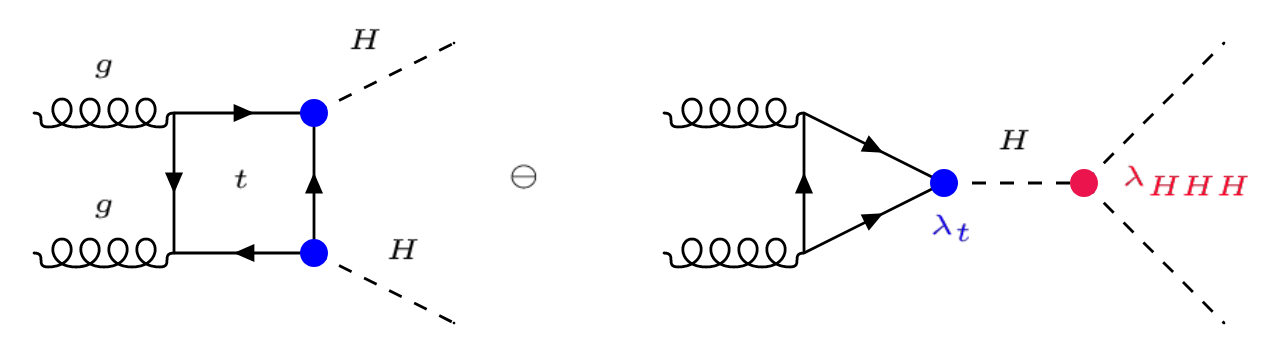
\includegraphics[width=0.8\textwidth]{Ch1/Img/HH_feyn.png}
    \caption{Leading Order (LO) Feynman diagrams contributing to ggF Higgs boson pair production through a top-quark loop (box) and through the triple self-coupling of the Higgs boson (triangle).}
    \label{fig:chap1:HH:HPD:FY}
\end{figure}
The SM cross-section for Higgs boson pair production via ggF at $\sqrt{s}=13$ TeV, calculated at Next-to-Next Leading Order (NNLO) \cite{HHXSec1, HHXSec2}, is:
\begin{equation}
    \sigma_{\text{ggF HH}}^{\text{NNLO}} = 31.05_{-5.0\%}^{+2.2\%} \ \text{fb},
    \label{eq:chap1:HH:XSEC:NNL0}
\end{equation}
three orders of magnitude smaller than the single Higgs boson production cross-section. This accounts for more than 90\% of the total Higgs boson pair production cross-section. VBF mode also contributes to the di-Higgs boson production with a lower cross-section of $\sigma_{\text{VBF HH}}^{\text{NNLO}} = 1.723_{-0.04\%}^{+0.03\%} \ \text{fb}$. 

Figure \ref{fig:chap1:HH:HPD:FYS} shows the other production modes contributing to Higgs boson pair production. The corresponding cross-section as a function of centre-of-mass energy is shown in Figure \ref{fig:chap1:HH:BSM:XSEC:S}.
\begin{figure}[htbp]
    \centering
    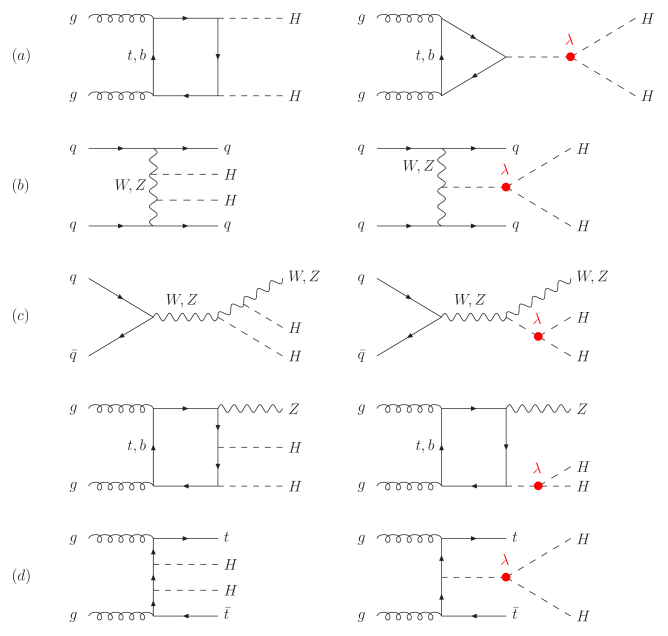
\includegraphics[width=0.65\textwidth]{Ch1/Img/HH_feyns.png}
    \caption{HH production modes, in decreasing order of cross-section. $\lambda$ referees to Higgs boson trilinear coupling: (a) ggF mode, (b) VBF mode, (c) Vector boson association (VH) and (d) top associated production.}
    \label{fig:chap1:HH:HPD:FYS}
\end{figure}
\\
Figure \ref{fig:chap1:HH:HPD:DCY} represents the matrix of the decay channels and their branching ratio of a pair of Higgs bosons resulting from all possible combination of decays of the two Higgs bosons. The dominant channels are $HH\rightarrow b\bar{b}b\bar{b}$, $HH\rightarrow b\bar{b}\tau\tau$ and $HH\rightarrow b\bar{b}WW^*$.
\begin{figure}[htbp]
    \centering
    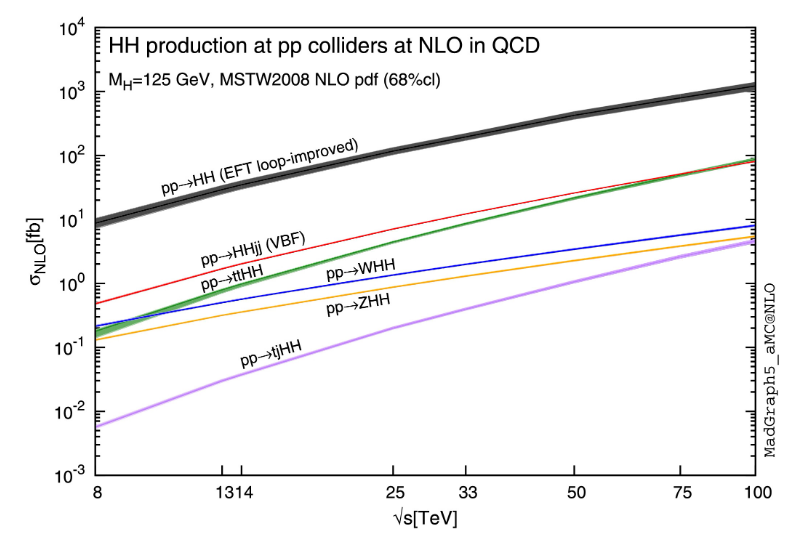
\includegraphics[width=0.5\textwidth]{Ch1/Img/HH_XSec_as_S.png}
    \caption{Total cross-sections at the NLO for HH production as a function of centre-of-mass energy. Assuming \kl and \kt equals to their SM values.}
    \label{fig:chap1:HH:BSM:XSEC:S}
\end{figure}
\begin{figure}[htbp]
    \centering
    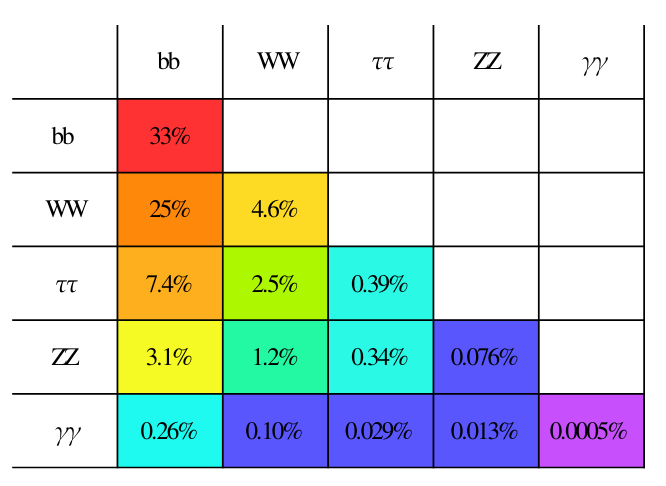
\includegraphics[width=0.5\textwidth]{Ch1/Img/HH_decays.png}
    \caption{Di-Higgs boson system decay branching ratios assuming SM Higgs bosons with $m_H=125.09$ GeV.}
    \label{fig:chap1:HH:HPD:DCY}
\end{figure}
\\
Even if there are other channels with branching ratios higher by one or two orders of magnitude, \bbyy final state is one of the most promising decay channels for the search for di-Higgs boson production as it has a good compromise between the large branching ratio from $H\to b\bar{b}$ decay and the small Higgs boson to diphoton branching ratio. The \bbyy channel is appealing thanks to an excellent diphoton invariant mass resolution leading to a clean diphoton signature through a narrow peak at Higgs boson mass in the $m_{\gamma\gamma}$ invariant mass spectrum on top of a smoothly falling background. This help to separate the signal from the background processes contrary to other channels such as \bbbb, $b\bar{b}WW^*$ and \bbtt. This thesis is performed on \bbyy final state.

\subsection{Di-Higgs boson as a probe of BSM physics}
\label{chap1:HH:BSM}
The small cross-section (Eq. \ref{eq:chap1:HH:XSEC:NNL0}) is making the di-Higgs boson observation challenging. 
If SM expectations hold, the production of a Higgs boson pair in a single $pp$ interaction should not be observed with the Run-2 data unless its cross-section is enhanced by an anomalous component (new physics). 
This makes HH a promising process to probe new physics beyond the standard model (BSM). 
Many of those BSM theories predict the existence of heavy particles that can decay into a pair of Higgs bosons. 
These could be identified as a resonance in the di-Higgs boson invariant mass spectrum. 
In addition to the resonant production, there can also be non-resonant scenarios which can bring substantial enhancement of the cross-section by modifying the relative sign of $\bigtriangleup$ and $\square$, and by increasing the $\bigtriangleup$ which is proportional to $\lambda_{HHH}$. Only the non-resonant search is considered in this thesis. These can either originate from loop corrections involving new particles, such as a light-coloured scalar, or through non-SM couplings. Anomalous couplings of Higgs boson with the top-quark or triple Higgs boson self-coupling can either be extensions to the SM, such as contact interactions between two top quarks and two Higgs bosons, or deviation from the SM values of the trilinear Higgs boson self-coupling. Considering possible modifications of them, the deviation is quantified by \kl $ = \frac{\lambda_{HHH}}{\lambda_{HHH}^{SM}}$ and \kt $= \frac{\lambda_{t}}{\lambda_{t}^{SM}}$, where $\lambda_{i}$ is the coupling $i$ of the new physics and $\lambda_{i}^{SM}$ its SM value. \\
Given the \kt and \kl modifiers, the Higgs boson pair production cross-section can be parameterized as:
\begin{equation}
  \sigma \approx k_{t}^{4}\left[|\square|^{2}+\frac{k_{\lambda}}{k_{t}}(\square\bigtriangleup+\bigtriangleup \square)+\left(\frac{k_{\lambda}}{k_{t}}\right)^{2}|\bigtriangleup|^{2}\right], 
  \label{eq:chap1:HH:XSEC:Param}
\end{equation}
this shows that the production cross-section depends on both parameters \kt and \kl, while the kinematics only depends on their ratio, that modifies the relative contribution of the two diagrams and thus the shape of the kinematic distributions. The maximum interference between the two diagrams corresponds to the cross-section minimum located at \kl = 2.4\kt. Figure \ref{fig:chap1:HH:BSM:I} shows an illustration of diagram contribution to the invariant mass distribution of di-Higgs boson system $m_{HH}$. The box diagram has an invariant mass spectrum peaking around 2$m_t$. When including the triangle diagram with the triple Higgs boson self-coupling, the invariant mass spectrum becomes generally softer with the increase of its contribution. This effect causes a large change in $m_{HH}$ distribution as shown in Figure \ref{fig:chap1:HH:BSM:MHH}.
\begin{figure}[htbp]
    \centering
    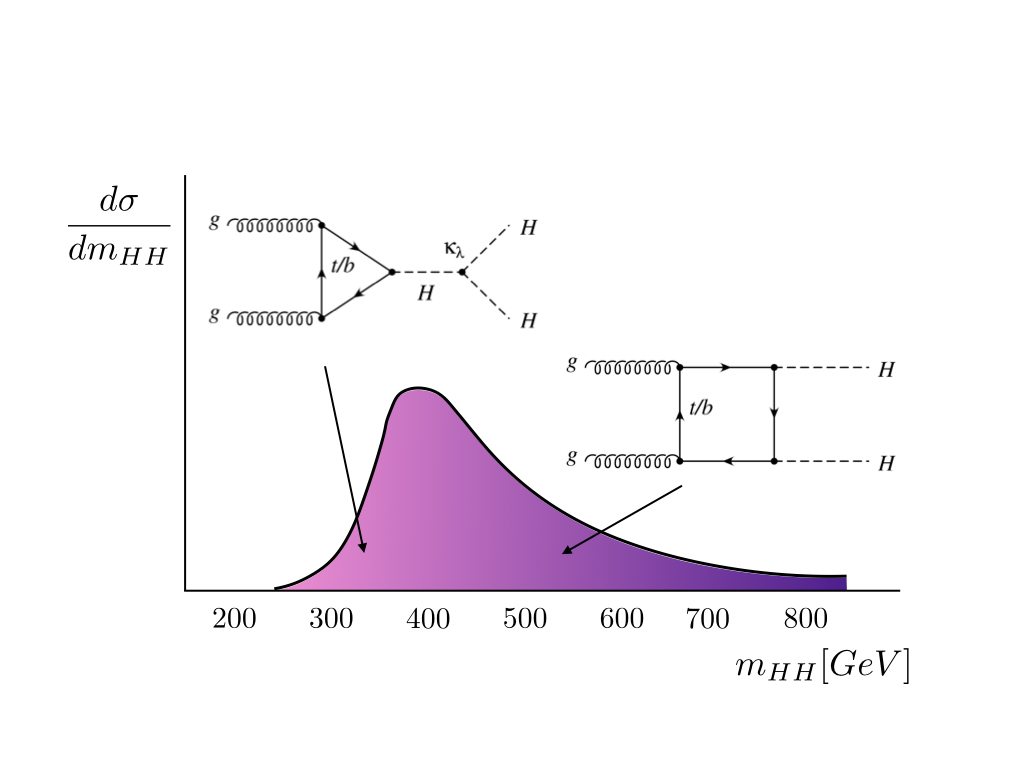
\includegraphics[width=0.5\textwidth]{Ch1/Img/illustration_mHH.jpeg}
    \caption{Illustration of both box and triangle diagrams contribution to di-Higgs boson invariant mass spectrum.}
    \label{fig:chap1:HH:BSM:I}
\end{figure}
The interference of the two diagrams also generates local minima in the differential cross-section around $m_{HH}=2m_t$ for the case of \kl = 2.
\begin{figure}[htbp]
    \centering
    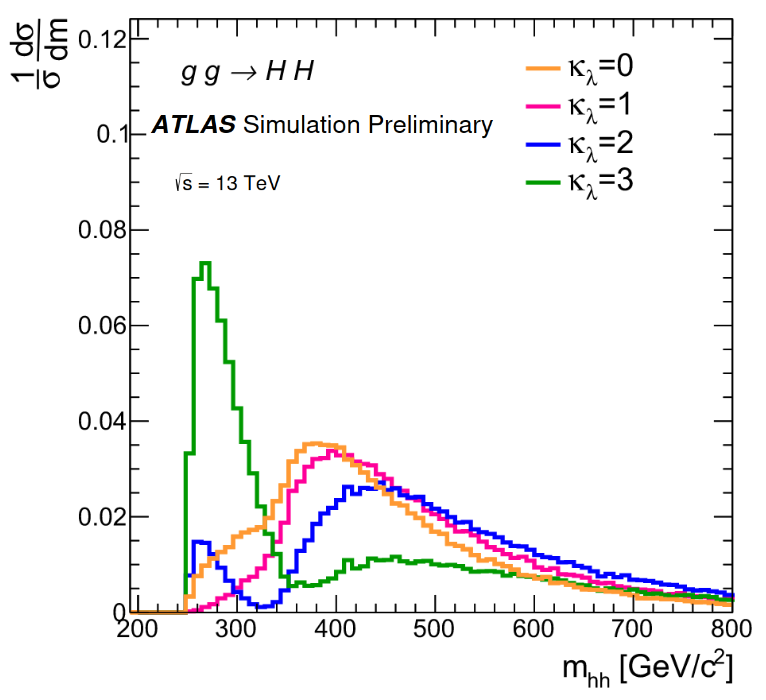
\includegraphics[width=0.5\textwidth]{Ch1/Img/mHH.png}
    \caption{Higgs boson pair invariant-mass distribution in ggF for various values of \kl assuming \kt = 1.}
    \label{fig:chap1:HH:BSM:MHH}
\end{figure}
Figure \ref{fig:chap1:HH:BSM:XSEC:L} displays the total LO and NLO cross-sections for the six dominant HH production channels at the LHC, as a function of the self-interaction coupling \kl.
\begin{figure}[htbp]
    \centering
    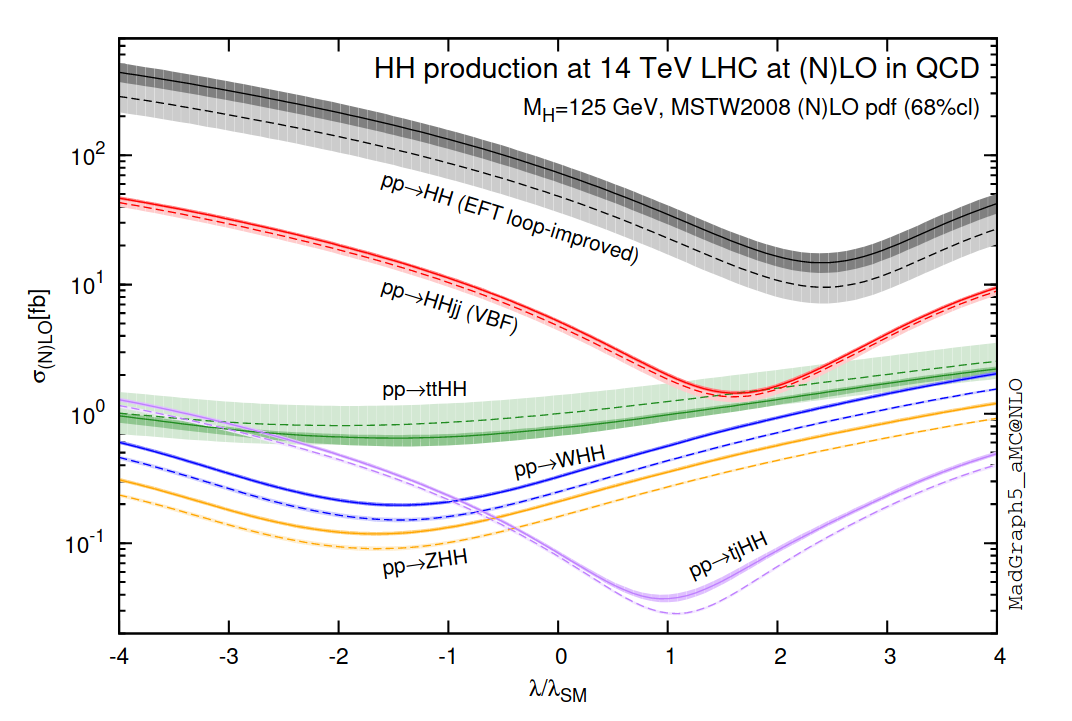
\includegraphics[width=0.5\textwidth]{Ch1/Img/HH_Xsec_as_lambda.png}
    \caption{The total LO and NLO cross-sections for HH production at $\sqrt{s}=14$ TeV, as a function of the self-interaction coupling \kl.}
    \label{fig:chap1:HH:BSM:XSEC:L}
\end{figure}
\\
As mentioned above, Higgs boson pair production is a promising process to probe new BSM physics. In this thesis, in addition to the search for the SM Higgs boson pair production process, constrain on \kl is also extracted. In this thesis, \kt is assumed to be one.

\subsection{Current measurements}
\label{chap1:HH:CM}
At the beginning of this thesis (2018), the latest measurement of Higgs boson pair cross-section in \HHyybb channel was performed based on dataset of 36 \ifb representing the data collected by ATLAS detector between 2015 and 2016 (Chapter \ref{LHC&ATLAS} is dedicated to ATLAS detector). Results of this analysis were consistent with the SM expectations \cite{yybb_36ifb}. The analysis set an observed (expected) upper limit at  95\% Confidence Level (CL) on HH production cross-section of 0.73 (0.93) pb, corresponding to 22 (28) times the predicted SM value. The Higgs boson self-coupling was constrained to be between -8.2 $<$ \kl $<$ 13.2 at 95\% CL (-8.3 $<$ \kl $<$ 13.2 expected), other SM parameters were fixed to their SM value when extracting limits. The limit scan as a function of \kl is shown in Figure \ref{fig:chap1:HH:CM:KL}. \\

\begin{table}[htbp]
    \centering
    \begin{tabular}{ccccc}
    \hline\hline
         & Observed & Expected & -1$\sigma$ & +1$\sigma$ \\
    \hline
        $\sigma_{gg\rightarrow HH}$ [pb] & 0.73 & 0.93 & 0.66 & 1.3 \\
        As a multiple of $\sigma_{SM}$ & 22 & 28 & 20 & 40 \\
    \hline\hline
    \end{tabular}
    \caption{The 95\% CL observed and expected limits on the Higgs boson pair cross-section in pb and as a multiple of the SM production cross-section. The $\pm1\sigma$ band around each 95\% CL limit is also indicated.}
    \label{tab:chap1:HH:CM:XSEC}
\end{table}
\begin{figure}[htbp]
    \centering
    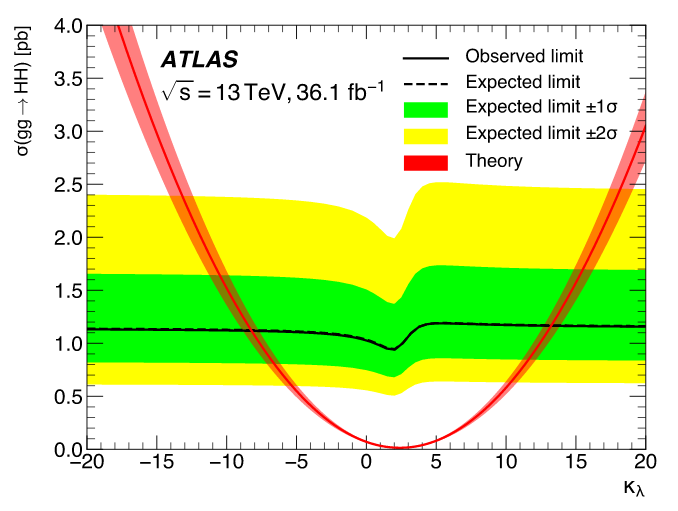
\includegraphics[width=0.5\textwidth]{Ch1/Img/kl_36ifb.png}
    \caption{The expected and observed 95\% CL limits on the non-resonant production cross-section $\sigma_{gg\rightarrow HH}$ as a function of $\kappa_{\lambda}$. The red line indicates the predicted HH cross-section as a function of \kl with all other couplings fixed at their SM values. The red band indicates the theoretical uncertainty of this prediction.}
    \label{fig:chap1:HH:CM:KL}
\end{figure}

Improving this measurement by contributing to the \HHyybb non-resonant analysis with the full Run-2 (2015-2018) data, and improve the current limits on the cross-section and constrain on the self-coupling is the aim of this thesis. 

%\section{Effective Field Theories (EFTs)}
%\label{chap1:EFT}
%In the context of the search for BSM physics, no indication has been found at the LHC. This could be explained by the fact that the new physics is not accessible at the LHC. Effective Field Theories (EFTs) provide an approach to probe the existence of BSM physics in a model-independent way at the LHC, even if the new physics scale $\Lambda$ is not directly accessible at the LHC. When BSM resides at scales larger than the EW scale ($\Lambda >> vev$), the new physics decouples from the SM and no light hidden states are produced. When this condition is satisfied, an expansion of the Lagrangian with canonical dimensions of $\frac{vev}{\lambda}$ can be performed. The theory that results is the Standard Model Effective Field Theory (SMEFT) \cite{SMEFT_EFT}. The SMEFT is well-defined and has been studied with increased theoretical sophistication in recent years, and it can capture a wide range of possible extensions of the SM. Such SM extensions can address the strong evidence for dark matter and neutrino masses not covered by SM. A linear EFT model of SMEFT is considered in this thesis:  
%\begin{equation}
%    \mathcal{L}_{S M E F T}=\mathcal{L}_{S M}+\mathcal{L}^{5}+\mathcal{L}^{6}+\mathcal{L}^{7}+\ldots, \quad \mathcal{L}^{d}=\sum_{i=1}^{n_{d}} \frac{C_{i}^{d}}{\Lambda^{d-4}} Q_{i}^{d} \quad for \ d>4.
%\end{equation}

%The number of non-redundant operators in $\mathcal{L}^i$ is known. The operators $Q_i^d$ are suppressed by d-4 powers of the cutoff scale $\Lambda$. These operators build a complete set of all operators allowed by the SM gauge symmetries. The Warsaw basis is used for the invariant operators $Q_i^d$ \cite{Warsaw}. The coefficients $C_i^d$ are called Wilson coefficients, which are free parameters of the theory. \\
%The new physics interferes with the SM, and modify the kinematic of the given process. The cross-section of a specific process within the SMEFT can be decomposed as: 
%\begin{equation}
%    \sigma = \sigma_{SM} + \sigma_{int} + \sigma_{BSM},
%\end{equation}
%where $\sigma_{SM}$ is the SM cross-section, $\sigma_{int}$ represents the interference between the BSM physics with the SM and $\sigma_{BSM}$ is a pure BSM physics suppressed by $\Lambda^{-4}$ that does not depend on the SM amplitude; it can, however, become important in specific regions of the phase space and its consideration can prevent negative cross-sections. \\

%Projecting measurements of the interactions of the known SM states into an effective field theory framework is an important goal of the LHC physics program \cite{LHC_EFT}. The interpretation of measurements of the properties of the Higgs boson in an EFT allows one to consistently study the properties of this state. Similarly to \kl variations, new physics can affect Higgs boson pair production. Higgs boson pair production results can benefit from a re-interpretation beyond the \kl variations. The full Run 2 di-Higgs boson results can be used to set limits on SMEFT operators that affect the HH production. Detailed studies of EFT within double Higgs boson context are described in the dedicated Chapter \textbf{To Be Added}.

\section{Conclusion}
\label{chap1:Conc}
The Higgs boson mechanism is a key component of the SM to explain the origin of the mass of the particles. A particle with similar properties to the SM Higgs boson was discovered at collisions of the LHC in 2012. After its discovery, a priority of the ATLAS and CMS collaborations has been to measure more precisely its properties and couplings. Understanding Higgs boson self-coupling is providing a direct probe on electroweak symmetry breaking (EWSB) and experimentally reconstruction of the Higgs potential. The theoretical backgrounds needed to understand the main subject of the thesis is introduced. The current HH search results with 2015-2016 data are also presented. %The EFT is highlighted as an interpretation of di-Higgs results beyond \kl. 
The next chapter focuses on the experimental setup to produce and collect data, the Large Hadron Collider and the ATLAS detector. 

